% Based on "sig-alternate.tex" V2.0 May 2012
% This file should be compiled with V2.5 of "sig-alternate.cls" May 2012
%
% This example file demonstrates the use of the 'sig-alternate.cls'
% V2.5 LaTeX2e document class file. It is for those submitting
% articles to ACM Conference Proceedings WHO DO NOT WISH TO
% STRICTLY ADHERE TO THE SIGS (PUBS-BOARD-ENDORSED) STYLE.
% The 'sig-alternate.cls' file will produce a similar-looking,
% albeit, 'tighter' paper resulting in, invariably, fewer pages.
%
% ----------------------------------------------------------------------------------------------------------------
% This .tex file (and associated .cls V2.5) produces:
%       1) The Permission Statement
%       2) The Conference (location) Info information
%       3) The Copyright Line with ACM data
%       4) NO page numbers
%
% as against the acm_proc_article-sp.cls file which
% DOES NOT produce 1) thru' 3) above.
%
% Using 'sig-alternate.cls' you have control, however, from within
% the source .tex file, over both the CopyrightYear
% (defaulted to 200X) and the ACM Copyright Data
% (defaulted to X-XXXXX-XX-X/XX/XX).
% e.g.
% \CopyrightYear{2007} will cause 2007 to appear in the copyright line.
% \crdata{0-12345-67-8/90/12} will cause 0-12345-67-8/90/12 to appear in the copyright line.
%
% ---------------------------------------------------------------------------------------------------------------
% This .tex source is an example which *does* use
% the .bib file (from which the .bbl file % is produced).
% REMEMBER HOWEVER: After having produced the .bbl file,
% and prior to final submission, you *NEED* to 'insert'
% your .bbl file into your source .tex file so as to provide
% ONE 'self-contained' source file.
%
% ================= IF YOU HAVE QUESTIONS =======================
% Questions regarding the SIGS styles, SIGS policies and
% procedures, Conferences etc. should be sent to
% Adrienne Griscti (griscti@acm.org)
%
% Technical questions _only_ to
% Gerald Murray (murray@hq.acm.org)
% ===============================================================
%
% For tracking purposes - this is V2.0 - May 2012

\documentclass{acm_proc_article-sp}

\begin{document}

\title{An Evaluation of Potential Reputation System Metrics for Android Applications and Application Developers}
%
% You need the command \numberofauthors to handle the 'placement
% and alignment' of the authors beneath the title.
%
% For aesthetic reasons, we recommend 'three authors at a time'
% i.e. three 'name/affiliation blocks' be placed beneath the title.
%
% NOTE: You are NOT restricted in how many 'rows' of
% "name/affiliations" may appear. We just ask that you restrict
% the number of 'columns' to three.
%
% Because of the available 'opening page real-estate'
% we ask you to refrain from putting more than six authors
% (two rows with three columns) beneath the article title.
% More than six makes the first-page appear very cluttered indeed.
%
% Use the \alignauthor commands to handle the names
% and affiliations for an 'aesthetic maximum' of six authors.
% Add names, affiliations, addresses for
% the seventh etc. author(s) as the argument for the
% \additionalauthors command.
% These 'additional authors' will be output/set for you
% without further effort on your part as the last section in
% the body of your article BEFORE References or any Appendices.

\numberofauthors{3} %  in this sample file, there are a *total*
% of EIGHT authors. SIX appear on the 'first-page' (for formatting
% reasons) and the remaining two appear in the \additionalauthors section.
%
\author{
% You can go ahead and credit any number of authors here,
% e.g. one 'row of three' or two rows (consisting of one row of three
% and a second row of one, two or three).
%
% The command \alignauthor (no curly braces needed) should
% precede each author name, affiliation/snail-mail address and
% e-mail address. Additionally, tag each line of
% affiliation/address with \affaddr, and tag the
% e-mail address with \email.
%
% 1st. author
\alignauthor
Theresa Guinard\\
       \affaddr{New Mexico Institute of Mining and Technology}\\
       \affaddr{801 Leroy Place}\\
       \affaddr{Socorro, New Mexico}\\
       \affaddr{1-(575)-835-5434}
       \email{tguinard@cs.nmt.edu}
% 2nd. author
\alignauthor
Randall Van Why\\
       \affaddr{New Mexico Institute of Mining and Technology}\\
       \affaddr{801 Leroy Place}\\
       \affaddr{Socorro, New Mexico, 87801}\\
       \affaddr{1-(575)-835-5434}
       \email{rvanwhy@cs.nmt.edu}
% 3rd. author
\and
\alignauthor
Dr. Jun Zheng\\
       \affaddr{New Mexico Institute of Mining and Technology}\\
       \affaddr{801 Leroy Place}\\
       \affaddr{Socorro, New Mexico, 87801}\\
       \affaddr{1-(575)-835-5434}
       \email{zheng@cs.nmt.edu}
% 3rd. author
%\alignauthor Lars Th{\o}rv{\"a}ld\titlenote{This author is the
%one who did all the really hard work.}\\
%       \affaddr{The Th{\o}rv{\"a}ld Group}\\
%       \affaddr{1 Th{\o}rv{\"a}ld Circle}\\
%       \affaddr{Hekla, Iceland}\\
%       \email{larst@affiliation.org}
%\and  % use '\and' if you need 'another row' of author names
%% 4th. author
%\alignauthor Lawrence P. Leipuner\\
%       \affaddr{Brookhaven Laboratories}\\
%       \affaddr{Brookhaven National Lab}\\
%       \affaddr{P.O. Box 5000}\\
%       \email{lleipuner@researchlabs.org}
%% 5th. author
%\alignauthor Sean Fogarty\\
%       \affaddr{NASA Ames Research Center}\\
%       \affaddr{Moffett Field}\\
%       \affaddr{California 94035}\\
%       \email{fogartys@amesres.org}
%% 6th. author
%\alignauthor Charles Palmer\\
%       \affaddr{Palmer Research Laboratories}\\
%       \affaddr{8600 Datapoint Drive}\\
%       \affaddr{San Antonio, Texas 78229}\\
%       \email{cpalmer@prl.com}
}
% There's nothing stopping you putting the seventh, eighth, etc.
% author on the opening page (as the 'third row') but we ask,
% for aesthetic reasons that you place these 'additional authors'
% in the \additional authors block, viz.
%\additionalauthors{Additional authors: John Smith (The Th{\o}rv{\"a}ld Group,
%email: {\texttt{jsmith@affiliation.org}}) and Julius P.~Kumquat
%(The Kumquat Consortium, email: {\texttt{jpkumquat@consortium.net}}).}
%\date{30 July 1999}
% Just remember to make sure that the TOTAL number of authors
% is the number that will appear on the first page PLUS the
% number that will appear in the \additionalauthors section.

\maketitle

\section{Introduction}
The current rating system for applications is antiquated. As more people adopt smartphones as their choice of mobile technology, it becomes increasingly
difficult for users to sift through reviews in order to determine how other users feel about a mobile application. In addition, the 5-star rating systems used in many modern markets are too coarse to describe accurate sentiment. Our goal is to develop a system that uses existing mobile application data in order to provide users with a better understanding of the reception of an app. 

\section{Background and Related Work}

In order to perform sentiment analysis, two approaches were taken: using SentiWordNet scores, and a support vector machine trained with star ratings.

Support Vector Machine (SVM) use in sentiment analysis has proven to be an effective approach to sentiment analysis, in comparison with other machine learning techniques \cite{Pang02thumbsup}.  When preprocessing input for an SVM, it is helpful to use WordNet lemmas.  WordNet is a lexical resource that groups English words into synonym sets, and words are tagged by part of speech \cite{Miller}.  To normalize the input, term frequency-inverse document frequency (tf-idf) can be used.  To reduce dimensionality, latent semantic analysis (LSA), which uses singular value decomposistion, can be used \cite{Deerwester90indexingby}.  This follows a simiar approach as \cite{Mullen04sentimentanalysis}

SentiWordNet is a dataset that assigns a sentiment score to members of WordNet.  Sentiment scores were generated using the structure of WordNet as well as the Princeton WordNet Gloss Corpus \cite{Baccianella10sentiwordnet}.

%Describe specialized and relevant related background necessary to appreciate the work.  Include references to the literature where appropriate, and briefly explain where your work departs from that done by others.  Reference lists do not count towards the limit on the length of the abstract.
%This is an example of a citation~\cite{Lamport:LaTeX}.

\section{Approach and Uniqueness}
%Describe your approach in attacking the problem and how your approach is novel.  Your hypothesis may be here.

\subsection{Sentiment Analysis}
One implemented sentiment analysis approach involved using SentiWordNet.  Part of speech tagging was performed on each review. The sum of SentiWordNet scores for adverbs, verbs, and adjectives was taken to determine whether the review was positive, negative, or neutral overall.  Each review was assigned a sentiment score of 1, -1, or 0 (positive, negative, or neutral), and each app received a sentiment score which was calculated by the proportion of positive to negative reviews.

Results were compared to another approach to sentiment analysis: using a support vector machine (SVM) trained using the ratings of a subset of the comments.  To transform the reviews into SVM input, the adjectives, adverbs, and verbs were considered (these were determined using part of speech tagging).  These words were lemmatized using WordNet, the comments were normalized via tf-idf, and to reduce the dimensionality of input, LSA was used.  A sample of one-star and five-star comments was taken from the corpus of reviews to train the SVM.

The advantage of the SVM approach is that it potentially handles domain-specific factors better, but it is also potentially non-extensible to comments of applications outside of the training set.  However, in this project, comments for the training set were taken from all applications, and the purpose of performing semantic analysis was primarily to classify the sentiments of the more neutrally-rate comments (2-4 stars).


\subsection{Application Metric Comparison}
Several metrics dealing with application quality are directly available from Google Play.  This includes approximate number of downloads, average 1-5 star rating, and whether the developer is a Top Developer.  In order to determine which metrics are useful in a rating system, these different metrics are compared across the top-downloaded applications, and we determine if there is any correlation.

\section{Results and Application}
There are many potential applications for the calculated sentiment score and other available metrics. One particularly interesting application is developer rating: using the aggregate sentiment scores of the applications created by a developer, we can generate a generalized ``reputation'' score that will attempt to measure the reliability of the developer.

This reputation score will provide much needed information about developer reliability which can be a dramatic improvement over the existing information. To elaborate, the Google Play store designates certain developers as ``Top Developers'' which is indicated via badges. However, being a ``Top Developer'' does not indicate that the developer has written a large number of apps or even that the apps are of good quality.
%\pagebreak
\begin{figure}[!h]
\centering

\epsfig{file=piggy.png,width=0.5\textwidth}
\caption{An example of a mediocre app from a Top Developer.}
\label{fig:myfig}
\end{figure} 

\subsection{Results}
%Provide an overview of results.  Use tables or figures as appropriate.  Place Tables/Figures/Images in text as close to the reference as possible, typically at the top of a column (see Figure~\ref{fig:myfig}).
For the sentiment analysis score, the SentiWordNet technique correlates with overall app rating more than the SVM technique does.  For predicting the sentiment of one- and five-star comments, the SVM technique is more accurate.

\begin{figure}[!h]
\centering
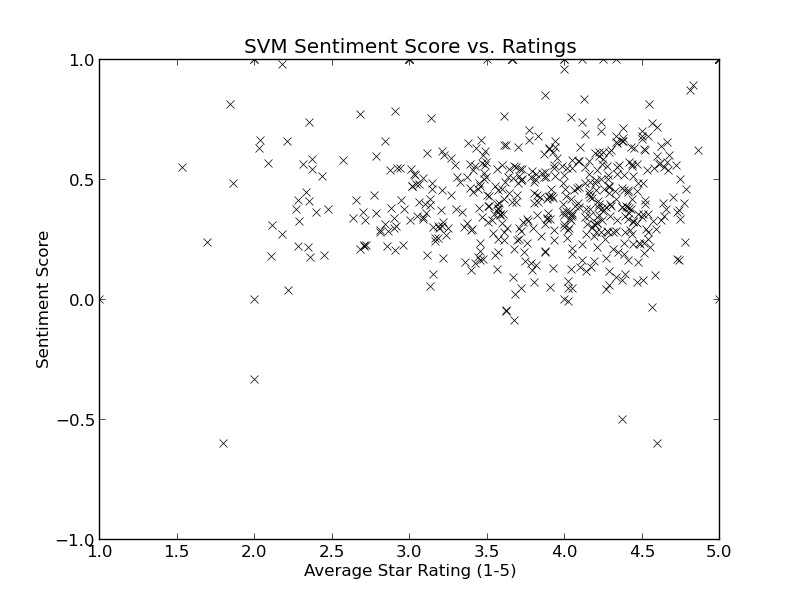
\epsfig{file=svm.png,width=0.5\textwidth}
\caption{SVM sentiment scores vs. average star ratings}
\label{fig:myfig1}
\end{figure}

\begin{figure}[!h]
\centering
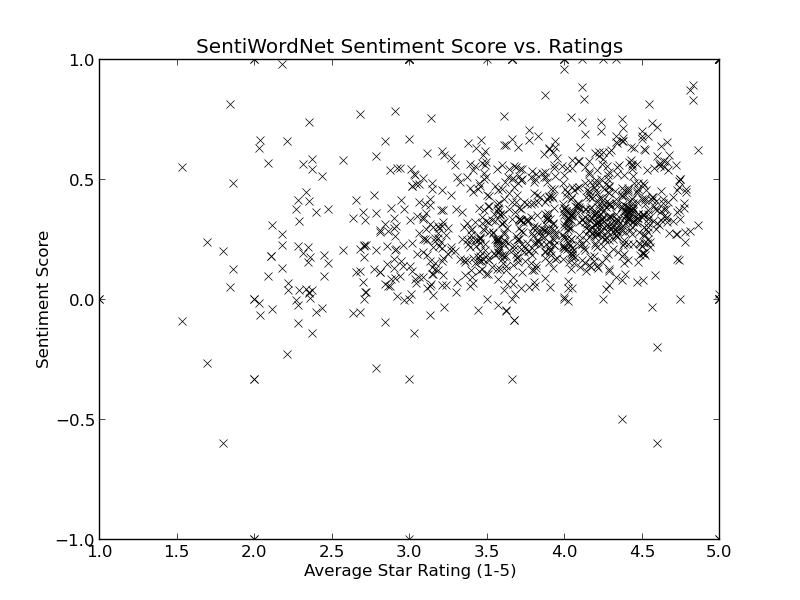
\epsfig{file=swn.png,width=0.5\textwidth}
\caption{SentiWordNet sentiment scores vs. average star ratings}
\label{fig:myfig2}
\end{figure}

\begin{table}[!h]
\centering
\caption{Accuracy of 1 and 5 star sentiment predictions}
\begin{tabular}{|c|c|}
\hline
& \textbf{Accuracy} \\ \hline
SVM & 0.735 \\ \hline
SentiWordNet & 0.709 \\ \hline
\end{tabular}
\end{table}

\subsection{Contributions}
This work contributes to the study of reputation systems by taking a critical look at the quality of various metrics.
\begin{itemize}
\item{We have compared existing sentiment analysis techniques, and evaluated their effectiveness for predicting the aggregate sentiment of an application from multiple reviews.}
\item{We have investigated corrrelations between multiple metrics that determine the quality of an application, which can be used to determine the overall quality of an application of an application developer.}
\end{itemize}

% The following two commands are all you need in the
% initial runs of your .tex file to
% produce the bibliography for the citations in your paper.
\bibliographystyle{abbrv}
\bibliography{sigproc}  % sigproc.bib is the name of the Bibliography in this case
% You must have a proper ".bib" file
%  and remember to run:
% latex bibtex latex latex
% to resolve all references

\balancecolumns
\end{document}
